\section{\wip Motivation and Aims}

\gls{latex}
\acrshort{fpt}

\begin{enumerate}
    \item What is the general problem?
    \begin{itemize}
        \item Parameterized Streaming Algorithms for k-VC
        \begin{enumerate}
            \item $2^k$-Pass BST using $O(k \cdot \text{log } n)$ bits
            % \begin{figure}[h]
            %     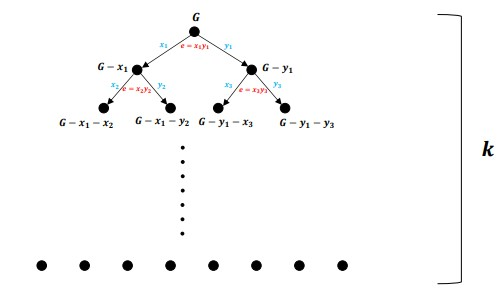
\includegraphics{2^k-pass-bst}
            %     \centering
            % \end{figure}
            \item $1$-Pass BST using $O(k^2 \cdot \text{log } n)$ bits
            \item Greedily maintain Maximal Matching $O(k^2)$ stored vertices and edges
            % \begin{figure}[h]
            %     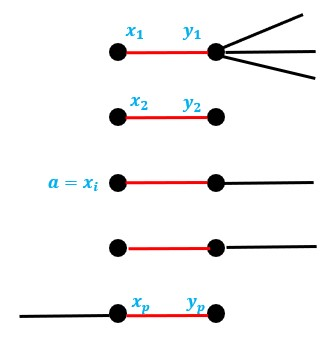
\includegraphics{1-pass}
            %     \centering
            % \end{figure}
            \item $O(k^2)$ Kernel
        \end{enumerate}
        \item \note{Copied from pdf}Recall that in the classical Vertex Cover problem, the goal is to find a min vertex cover. In the parameterized Vertex Cover problem, given a parameter k, we only want to know if $G$ has a vertex cover of size $\leq k$ or not. The goal is to develop fast algorithms when $k$ is small, even if the input size $n$ is large.
        \item Definition: A parameterized problem with parameter $k$ and input size $n$ is said to be fixed-parameter tractable (FPT) if it can be solved in time $f(k) \cdot n^{O(1)}$, for some function $f$.
    \end{itemize}
    \item Why is it worth working on?
    \begin{itemize}
        \item Graphs have been shown to be excellent models for real world situations
        \item Having a low enough algorithmic complexity to be able to solve some problems on graphs allows us to solve real world problems
    \end{itemize}
    \item Who else as worked on this problem?
    \begin{itemize}
        \item Rajesh Chitnis et al
    \end{itemize}
    \item What did they find?
    \begin{itemize}
        \item That this works in theory
    \end{itemize}
    \item Given this, what is the specific problem you will solve?
    \begin{itemize}
        \item Showing their performance vs real world datasets
    \end{itemize}
\end{enumerate}

\todo[inline]{Talk more about the work Rajesh has done}

My supervisor Rajesh Chitnis had previously been researching the problem of parameterized vertex cover. I found that none of the algorithms he talked about had ever been put into practice, only ever written theoretically.

\subsection{The Problem}
\subsection{Why Bother?}
\subsection{Previous Contributions}
\subsection{What I Plan To Contribute}
